\section{Evaluation and Discussion}

\begin{figure}
    \centering
    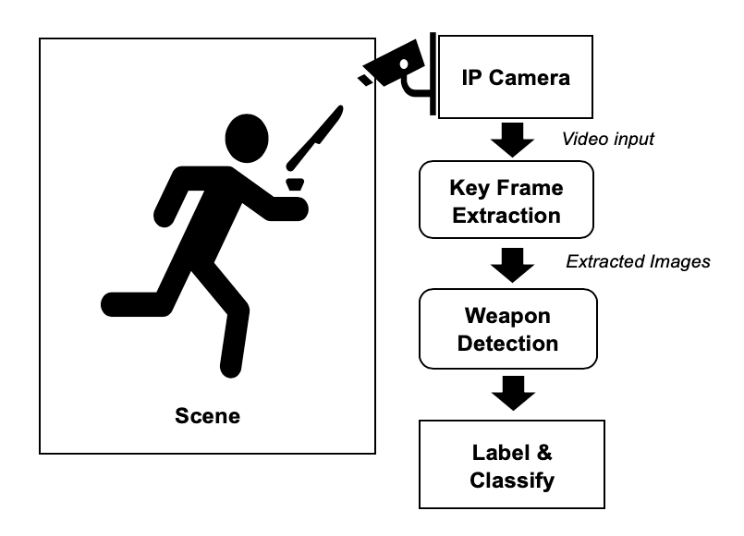
\includegraphics[width=6cm]{Security Object Detection, Surveillance/Latex/figures/fig5.png}
    \caption{Functional blocks of the proposed system \cite{Xu}}
    \label{fig:fig5}
\end{figure}

We used human detection by implementing Convolutional Neural Network (CNN) since is the most widely used deep learning technology, and it performs very well in the fields of image classification and object detection \cite{Xie}. This allowed us to use existing libraries that have been trained to detect people at a distance without interfering with the other functions of a camera system. CNN is basically basically several layers staged together just like another neural network structure \cite{Dinama}. A layer consists of linear filters which is followed by a non-linear activation function. A pooling layer then followed by convolutional layer. Max pooling is simply taking the maximum value from predetermined window. Additoinally, CNN is composed of mesh segmentation. From a machine learning  point of view, mesh segmentation can be broadly categorised as unsupervised and supervised segmentation \cite{George}. It requires a higher level understanding of the 3D
shapes, as composition of an object often relates to shapes and functionality of its parts. This allows for fully connected neural networks, NN. It consist of several fully
connected layers followed by a classification layer to produce prediction
probabilities. 

COCO object detection was used as shown in figure \ref{fig:fig4}. Fine tuning can result in a more efficient model. The COCO dataset consists of 328 000 images, of which there are 2.5 million labelled instances, and about 90 categories \cite{Pienaar}. After having satisfactory test results, it is possible to to export a photo file or live video to use for  object detection. Furthermore, CNN can also be used to detect potentially dangerous intruders equipped with firearms. Figure \ref{fig:fig5} shows the functional blocks of the proposed system. After the video is captured by the surveillance camera, it is passed to the key frame extraction subsystem, which reduces data size by selecting key frames for feasible real-time running of the subsequent steps \cite{Xu}. Additionally, techniques can be developed to increase the efficiency of human detection, such as at night. For example, an algorithm can be based on the fact that thermal images produced by thermal cameras make it possible to see any environment with or without light. The amount of radiation emitted by an object increases
with the temperature and the variations in temperature can be visualized for detecting a person \cite{Sharma}.

Figure \ref{fig:fig6} demonstrates how a night vision algorithm can be implemented. This can be useful to add extra functionally to our existing algorithm. This is what is fascinating about CNN, it can be expanded upon and improved to meet different use cases. Now, instead of having just a regular daytime surveillance system, a person can have a system where it does multiple functions, such as detecting a person and determining if a weapon is being carried. Additionally, the system can be setup to alert the user if it detects certain parameters. Our algorithm is more modest, focusing on the detection of humans with expandability in mind for future updates.

\begin{figure}
    \centering
    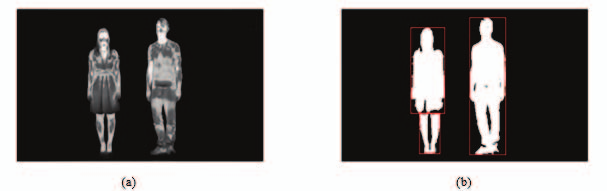
\includegraphics[width=6cm]{Security Object Detection, Surveillance/Latex/figures/fig6.png}
    \caption{(a) is the original image and (b) is binary with human detected \cite{Sharma}}
    \label{fig:fig6}
\end{figure}

\begin{figure}
    \centering
    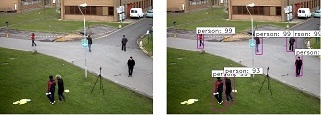
\includegraphics[width=8.5cm]{Security Object Detection, Surveillance/Latex/figures/fig4.jpg}
    \caption{Detection result of training algorithm \cite{Dinama}}
    \label{fig:fig4}
\end{figure}

 